\documentclass[12pt,a4paper]{article}
\usepackage[utf8]{inputenc}
\usepackage[spanish]{babel}
\usepackage{amsmath}
\usepackage{amsfonts}
\usepackage{amssymb}
\usepackage{graphicx}
\usepackage[left=2cm,right=2cm,top=2cm,bottom=2cm]{geometry}

\usepackage{enumitem}
\usepackage{algorithm}
\usepackage{algorithmic}
\usepackage[hidelinks]{hyperref}

\usepackage{subcaption}
\usepackage{pgfplots}

% Para la tabla
\usepackage[normalem]{ulem}
\useunder{\uline}{\ul}{}


\author{Ignacio Aguilera Martos}
\title{Práctica 2 \\ Aprendizaje Automático}
\date{22 de Abril de 2019}

\setlength{\parindent}{0cm}
\setlength{\parskip}{10px}


\begin{document}
	\maketitle

	\tableofcontents

	\newpage

\section{Ejercicio 1}

\subsection{Apartado 1}

Dibujemos en primer lugar la gráfica que se nos pide tanto con una uniforme como con una distribución normal o gaussiana.

\begin{figure}
	\centering
	\begin{subfigure}{0.47\textwidth}
		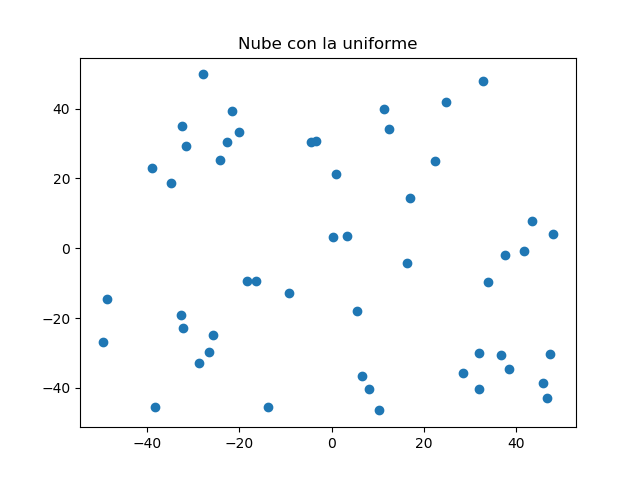
\includegraphics[scale=0.55]{./Imagenes/ej1-1.png}
		\caption{Nube generada con una uniforme}
	\end{subfigure}
	\begin{subfigure}{0.47\textwidth}
		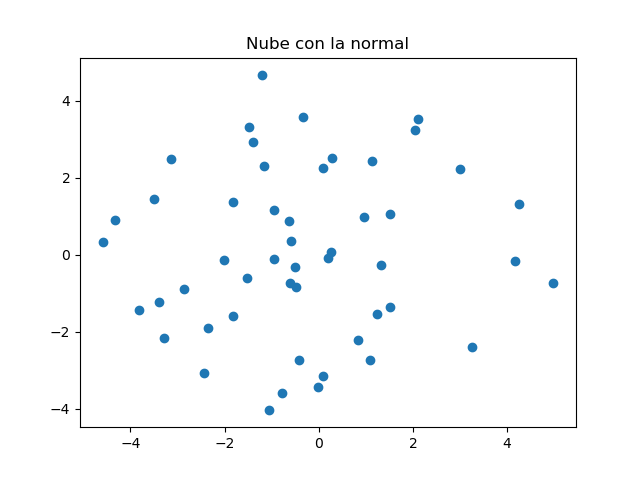
\includegraphics[scale=0.55]{./Imagenes/ej1-2.png}
		\caption{Nube generada con una normal}
	\end{subfigure}
\end{figure}

Podemos observar que el comportamiento de generación de puntos es completamente distinto. En el caso de la uniforme los puntos se generan de forma aleatoria de forma que la probabilidad de sacar un punto es la misma para todos los del cuadrado. Esto es, en la generación de datos el punto $(-40,40)$ y $(20,16)$ tienen la misma probabilidad de ser elegidos. Esto no es así en el caso de la uniforme. En este caso la probabilidad de escoger un punto es mayor a medida que nos acercamos al centro del cuadrado. Es por esto que podemos ver una concentración de los puntos en el centro y no en las esquinas.

\section{Ejercicio 2}

\section{Bonus}


\end{document}
